\subsection{パラメータ同定、周波数応答測定、実験計画}

MPC、オブザーバ、制御配分を実装するには、制御対象の式だけでなく、式に入るパラメータが必要である。質量、時定数、摩擦係数、ゲイン、むだ時間、センサのスケール係数は設計値から始められるが、実機では部品差、温度、摩耗、取付け条件によりずれる。パラメータ同定とは、入力 $u$、出力 $y$、必要なら状態 $x$ の測定記録から、モデル
\begin{equation}
  x_{k+1}=f(x_k,u_k,\theta),
  \qquad
  y_k=h(x_k,u_k,\theta)
\end{equation}
または低次の入出力モデルに含まれる未知量 $\theta$ を推定することである。同定したモデルは制御器を作るためのデータであり、同じデータだけで性能を判断してはならない。設計用の同定データと、別に取得した検証データを分けることが、実装時の最小条件である。

\subsubsection{ステップ、インパルス、正弦波実験による低次モデル}

同定実験は、まず運転点を定めることから始める。入力、出力、状態の定常値を $u_0,y_0,x_0$ とし、実験中の偏差を
\begin{equation}
  \tilde{u}=u-u_0,
  \qquad
  \tilde{y}=y-y_0,
  \qquad
  \tilde{x}=x-x_0
\end{equation}
と書く。線形同定で得られるモデルは、この運転点の近くで成り立つ小信号モデルである。入力の振幅を大きくしすぎると信号対雑音比は良くなるが、飽和、摩擦、温度変化、幾何的非線形性により一つの線形モデルでは表せなくなる。逆に振幅が小さすぎると、測定ノイズと量子化に埋もれてパラメータが不安定になる。

一次遅れとむだ時間を持つ安定な対象を
\begin{equation}
  G(s)=\frac{K}{Ts+1}e^{-Ls}
\end{equation}
で近似する。$K$ は静的ゲイン、$T$ [s] は時定数、$L$ [s] はむだ時間である。入力に大きさ $\Delta u$ のステップを入れ、$t\ge L$ で
\begin{equation}
  \tilde{y}(t)\simeq K\Delta u\left(1-e^{-(t-L)/T}\right)
\end{equation}
と応答するなら、十分時間が経った出力変化 $\Delta y_\infty$ から
\begin{equation}
  \hat{K}=\frac{\Delta y_\infty}{\Delta u}
\end{equation}
を得る。むだ時間 $L$ を差し引いた後、出力が最終変化量の $1-e^{-1}\simeq0.632$ に達する時刻が時定数 $T$ の推定値になる。ただし、二次以上の対象、零点を持つ対象、積分要素を持つ対象では、この読取りだけでは不十分である。ステップ応答は実装しやすいが、主に低周波と定常ゲインを強く励起する実験であり、帯域全体のモデルを決めるものではない。

幅の狭いパルス入力は、面積
\begin{equation}
  A_u=\int_0^{\tau_p}\tilde{u}(t)\,\dd t
\end{equation}
を持つ近似インパルスとして扱える。パルス幅 $\tau_p$ が対象の主要時定数より十分短ければ、一次遅れの応答は
\begin{equation}
  \tilde{y}(t)\simeq A_u\frac{K}{T}e^{-(t-L)/T}
  \qquad (t\ge L)
\end{equation}
となる。インパルス実験は多くの周波数成分を同時に含むが、実機では入力ピークが大きくなりやすく、安全制限やアクチュエータのレート制限にすぐ触れる。そのため、実装では真のインパルスではなく、小さなパルス列または PRBS に置き換えることが多い。

正弦波実験では、運転点まわりで
\begin{equation}
  \tilde{u}(t)=a\sin\omega t
\end{equation}
を加え、過渡成分が減衰した後の出力を
\begin{equation}
  \tilde{y}(t)=b\sin(\omega t+\phi)
\end{equation}
と近似する。このとき、その周波数での周波数応答は
\begin{equation}
  \hat{G}(j\omega)=\frac{b}{a}e^{j\phi}
\end{equation}
である。一次遅れモデルなら
\begin{equation}
  \abs{G(j\omega)}
  =\frac{K}{\sqrt{1+(\omega T)^2}},
  \qquad
  \angle G(j\omega)=-\tan^{-1}(\omega T)-\omega L
\end{equation}
を複数の $\omega$ で合わせることにより、$K,T,L$ を同時に推定できる。ステップ実験が時間領域の低次特徴を与え、正弦波実験が制御帯域付近のゲインと位相を直接与える、と役割を分けて使う。

\subsubsection{最小二乗法による入出力モデルの推定}

測定列を使ってパラメータを機械的に求める基本形は最小二乗法である。線形離散時間の入出力モデルとして、遅れ $d$ を含む ARX 形
\begin{equation}
  y_k+a_1y_{k-1}+\cdots+a_{n_a}y_{k-n_a}
  =
  b_0u_{k-d}+b_1u_{k-d-1}+\cdots+b_{n_b}u_{k-d-n_b}+e_k
\end{equation}
を考える。$e_k$ はモデル化できなかった成分と測定ノイズをまとめた残差である。この式を
\begin{equation}
  y_k=\varphi_k^\T \theta+e_k
\end{equation}
と書くために
\begin{align}
  \varphi_k&=
  \begin{bmatrix}
    -y_{k-1}&\cdots&-y_{k-n_a}&u_{k-d}&\cdots&u_{k-d-n_b}
  \end{bmatrix}^\T,\\
  \theta&=
  \begin{bmatrix}
    a_1&\cdots&a_{n_a}&b_0&\cdots&b_{n_b}
  \end{bmatrix}^\T
\end{align}
と置く。$N$ 個のサンプルを積み重ねると
\begin{equation}
  Y=\Phi\theta+E
\end{equation}
である。二乗残差
\begin{equation}
  J(\theta)=\frac{1}{2}\norm{Y-\Phi\theta}^{2}
\end{equation}
を最小にする条件は
\begin{align}
  \frac{\pp J}{\pp\theta}
  &=-\Phi^\T (Y-\Phi\theta)=0,\\
  \Phi^\T \Phi\,\theta&=\Phi^\T Y
\end{align}
であり、$\Phi^\T \Phi$ が正則なら
\begin{equation}
  \hat{\theta}=(\Phi^\T \Phi)^{-1}\Phi^\T Y
\end{equation}
を得る。正則性は、入力と初期条件が十分に多様な方向を励起していることを要求する。たとえば、入力を一定値に保ったデータだけでは動特性の係数を分離できない。これを持続的励起の条件という。

測定ノイズの分散が時刻ごとに異なる場合や、外れ値を弱めたい場合には、重み付き最小二乗
\begin{equation}
  J_W(\theta)
  =\frac{1}{2}(Y-\Phi\theta)^\T W(Y-\Phi\theta),
  \qquad W=W^\T>0
\end{equation}
を使う。解は
\begin{equation}
  \hat{\theta}_W=(\Phi^\T W\Phi)^{-1}\Phi^\T WY
\end{equation}
である。さらに、物理的に不自然な大きい係数を避けたいときは正則化を加え、
\begin{equation}
  J_\rho(\theta)
  =\frac{1}{2}\norm{Y-\Phi\theta}^{2}
  +\frac{\rho}{2}\norm{\theta-\theta_0}^{2}
\end{equation}
を最小化する。ここで $\theta_0$ は設計値または事前に妥当と考える値であり、$\rho>0$ は測定データと事前情報の重みを決める。解は
\begin{equation}
  \hat{\theta}_\rho
  =(\Phi^\T \Phi+\rho I)^{-1}(\Phi^\T Y+\rho\theta_0)
\end{equation}
である。これは悪条件な同定問題を安定化するが、正則化を強くしすぎると実測データより事前値へ寄ったモデルになる。

状態が測れる場合には、状態空間モデルの行列を同じ考えで推定できる。線形離散モデル
\begin{equation}
  x_{k+1}=A_dx_k+B_du_k+w_k
\end{equation}
に対し、
\begin{equation}
  X_+=MZ+W,
  \qquad
  M=\begin{bmatrix}A_d&B_d\end{bmatrix},
  \qquad
  Z=
  \begin{bmatrix}
    x_0&x_1&\cdots&x_{N-1}\\
    u_0&u_1&\cdots&u_{N-1}
  \end{bmatrix}
\end{equation}
と積み重ねれば、
\begin{equation}
  \hat{M}=X_+Z^\T(ZZ^\T)^{-1}
\end{equation}
である。ただし、状態推定値を $x_k$ として使う場合には、推定誤差が回帰変数にも入る。入力だけに雑音がないという単純な最小二乗の仮定が崩れるため、残差の相関、推定器の遅れ、閉ループフィードバックによるバイアスを確認する必要がある。

\subsubsection{正弦波掃引と PRBS による周波数応答測定}

周波数応答測定では、制御帯域と共振帯域を直接確認する。正弦波掃引では、角周波数 $\omega_i$ を対数間隔で選び、各周波数で数周期分の過渡を待ってから記録する。入力を $a_i\sin\omega_i t$ とし、記録区間の出力を
\begin{equation}
  y(t_\ell)=c+\alpha\sin\omega_i t_\ell+\beta\cos\omega_i t_\ell+r_\ell
\end{equation}
で最小二乗近似する。係数から
\begin{equation}
  b_i=\sqrt{\alpha^2+\beta^2},
  \qquad
  \phi_i=\operatorname{atan2}(\beta,\alpha)
\end{equation}
を求めれば、
\begin{equation}
  \hat{G}(j\omega_i)=\frac{b_i}{a_i}e^{j\phi_i}
\end{equation}
である。定数項 $c$ を同時に推定するのは、測定区間中のオフセットを出力振幅へ混ぜないためである。低い周波数では一周期が長く、温度ドリフトや外乱が入りやすい。高い周波数ではサンプリング、アクチュエータの帯域、センサフィルタの位相遅れが支配的になる。したがって、掃引範囲は制御で使いたい帯域の少し上までにし、機械共振や入力上限へ近づく周波数では振幅を下げる。

PRBS、すなわち疑似ランダム二値信号は、入力を $+a$ と $-a$ の間で切り替え、多くの周波数成分を一度に含ませる実験信号である。離散フーリエ変換を使って、記録された入力と出力を
\begin{equation}
  U(\Omega_i),\qquad Y(\Omega_i)
\end{equation}
と書くと、単純な推定は
\begin{equation}
  \hat{G}(e^{j\Omega_i})
  =\frac{Y(\Omega_i)}{U(\Omega_i)}
\end{equation}
である。ただし、ノイズがある実測では、複数区間に分けて平均したスペクトルから
\begin{equation}
  \hat{G}(e^{j\Omega})
  =
  \frac{\widehat{S}_{yu}(\Omega)}
       {\widehat{S}_{uu}(\Omega)}
\end{equation}
と推定する方が安定する。$\widehat{S}_{yu}$ は出力と入力のクロススペクトル、$\widehat{S}_{uu}$ は入力の自己スペクトルである。PRBS は短時間で広い帯域を励起できるが、対象が非線形なら、同時に入った複数周波数の相互変調が生じる。入力振幅を小信号範囲に保ち、飽和、レート制限、デッドゾーンをまたぐデータを別扱いにする必要がある。

閉ループ中に同定する場合には、入力 $u_k$ が出力 $y_k$ から作られるため、外乱や測定ノイズが入力にも相関して入る。開ループで安全に実験できる対象なら、まず開ループで低振幅の応答を測る。開ループが不安定、または安全上閉ループを切れない対象では、参照信号や既存制御器の入力に小さな励起を重ねる。このとき推定対象は、対象単体の $G$ ではなく、閉ループ感度や補償器を含む信号経路になる。どの点に励起を入れ、どの点を測ったかをブロック線図として残さなければ、得られた周波数応答を設計モデルへ正しく戻せない。

\subsubsection{実験計画、安全制限、検証データ分割}

同定実験の品質は、後から計算で補えない。実験計画では、少なくとも次を事前に決める。第一に、同定するモデルの使用範囲である。MPC が使う運転点、状態範囲、入力範囲、温度範囲を明確にし、その範囲を代表するデータを取る。第二に、励起信号である。入力は推定したい次数と帯域を励起しなければならない。一次遅れのゲインだけならステップで足りるが、共振、むだ時間、入力遅れ、下位ループの帯域を知るには正弦波掃引や PRBS が必要である。第三に、信号対雑音比、すなわち SNR である。入力振幅 $a$ に対して出力振幅がノイズ標準偏差 $\sigma_y$ と同程度なら、位相とゲインの推定は大きく揺れる。設計上必要な周波数で、概ね
\begin{equation}
  \frac{b}{\sigma_y}
\end{equation}
が十分大きくなる振幅を選ぶ。ただし、安全余裕と線形範囲を越えてはならない。

安全制限は、測定後の注意ではなく、実験入力を生成する前に制約として入れる。状態安全集合を $\mathcal{X}_{\mathrm{safe}}$、入力集合を $\mathcal{U}_{\mathrm{safe}}$ とする。実験入力列は
\begin{equation}
  x_k\in\mathcal{X}_{\mathrm{safe}},
  \qquad
  u_k\in\mathcal{U}_{\mathrm{safe}},
  \qquad
  \abs{u_k-u_{k-1}}\le\Delta u_{\max}
\end{equation}
を満たす範囲で作る。さらに、実験中に停止する条件を
\begin{equation}
  h_j(x_k)>h_{j,\mathrm{stop}},
  \qquad
  \abs{r_k}>r_{\mathrm{stop}},
  \qquad
  q_k=0
\end{equation}
のように明示する。$r_k$ は監視残差、$q_k$ はセンサ、通信、計算締切などの健全性を表すフラグである。停止条件を実験者の判断に任せると、データの再現性だけでなく安全余裕の検証も失われる。

取得したデータは、同定用、検証用、必要なら最終確認用に分ける。同定用データで $\hat{\theta}$ を求め、同じデータの残差だけを小さくしても、モデルが将来の入力へ当たるとは限らない。検証用データでは、入力列をモデルへ入れて
\begin{equation}
  \hat{y}_{k|0}(\hat{\theta})
\end{equation}
を自由応答または一歩先予測として計算し、実測 $y_k$ と比較する。代表的な指標は
\begin{equation}
  \mathrm{RMSE}
  =
  \sqrt{\frac{1}{N}\sum_{k=1}^{N}(y_k-\hat{y}_{k|0})^2}
\end{equation}
と、平均を引いた実測変動に対する適合率
\begin{equation}
  \mathrm{fit}
  =
  1-
  \frac{\sqrt{\sum_k(y_k-\hat{y}_{k|0})^2}}
       {\sqrt{\sum_k(y_k-\bar{y})^2}}
\end{equation}
である。残差
\begin{equation}
  \varepsilon_k=y_k-\hat{y}_{k|0}
\end{equation}
が入力と相関して残るなら、入力から出力へ説明されていない動特性がある。残差の自己相関が長く残るなら、モデル次数が不足している、むだ時間がずれている、または外乱モデルが必要である。検証データで不合格になった場合は、同じ検証データを使って何度もモデルを調整すると、検証データも事実上の同定データになる。最終性能を確認するためには、調整に使っていない別データまたは別日条件を残す。

\subsubsection{一次遅れ温度系の同定例}

低次モデル同定の流れを、加熱入力と温度出力を持つ一次遅れ系で確認する。運転点を $u_0=0.30$、$y_0=25\,^\circ\mathrm{C}$ とし、入力を $\Delta u=0.20$ だけ増やした。十分時間が経った温度変化が $\Delta y_\infty=4.0\,\mathrm{K}$ であったなら、
\begin{equation}
  \hat{K}=\frac{4.0}{0.20}=20\,\mathrm{K}
\end{equation}
である。ここで入力 $u$ は 0 から 1 までの無次元指令なので、$K$ の単位は入力指令 1 あたりの温度変化である。温度変化が $0.632\Delta y_\infty=2.53\,\mathrm{K}$ に達した時刻が、むだ時間を差し引いて $50\,\mathrm{s}$ であったとする。このとき
\begin{equation}
  \hat{T}=50\,\mathrm{s}
\end{equation}
であり、連続時間モデルは
\begin{equation}
  \tilde{G}(s)=\frac{20}{50s+1}
\end{equation}
となる。

サンプリング周期を $T_s=5\,\mathrm{s}$ としてゼロ次ホールドで離散化すると、一次遅れは
\begin{equation}
  \tilde{y}_{k+1}=a\tilde{y}_k+b\tilde{u}_k
\end{equation}
と書ける。ただし
\begin{align}
  a&=e^{-T_s/T}=e^{-0.1}\simeq0.905,\\
  b&=K(1-a)\simeq20(1-0.905)=1.90
\end{align}
である。別に取得した小振幅 PRBS データから同じ形の回帰
\begin{equation}
  \tilde{y}_{k+1}=
  \begin{bmatrix}
    \tilde{y}_k&\tilde{u}_k
  \end{bmatrix}
  \begin{bmatrix}
    a\\b
  \end{bmatrix}
  +e_k
\end{equation}
を作り、最小二乗で $\hat{a},\hat{b}$ を求める。もし $\hat{a}=0.90$、$\hat{b}=1.85$ 程度であれば、ステップ読取りと PRBS 同定は整合している。さらに、角周波数 $\omega=0.02\,\mathrm{rad/s}$ の正弦波入力を振幅 $a_u=0.10$ で加えると、一次遅れモデルは
\begin{align}
  b_y
  &=a_u\frac{K}{\sqrt{1+(\omega T)^2}}
    =0.10\frac{20}{\sqrt{2}}
    \simeq1.41\,\mathrm{K},\\
  \phi&=-\tan^{-1}(1)=-45^\circ
\end{align}
を予測する。実測の振幅と位相がこの値から大きく外れるなら、時定数が一つでは足りない、むだ時間がある、センサフィルタの遅れが入っている、または運転点がずれている可能性がある。

この例で重要なのは、ステップ、PRBS、正弦波を同じモデルへ押し込むことではなく、互いに異なる観点で矛盾を調べることである。ステップは静的ゲインと主要時定数、PRBS は広い帯域の入出力関係、正弦波は設計帯域のゲインと位相を確認する。一次遅れ温度系では、ステップ読取りから $a\simeq0.905$、$b\simeq1.90$、PRBS 最小二乗から $\hat{a}=0.90$、$\hat{b}=1.85$ が得られているので、係数差は $\abs{\hat{a}-a}\simeq0.005$、$\abs{\hat{b}-b}\simeq0.05$ と小さい。この一致は、静的ゲインと主要時定数が大きく外れていないことを示す。一方で、MPC に入れるモデルは一段先の係数だけでなく、地平線全体の予測誤差、推定器が見る残差の構造、実装時の制約余裕を同時に支える。したがって、$a,b$ が近いという事実だけで採用を決めると、むだ時間、センサフィルタ、運転点ずれ、高次遅れを見落とし、\wfig{implementation-effects-examples} の制約余裕を過大評価する。

別日の検証データ $N=240$ 点に対して、同じ一次遅れモデルの残差を
\begin{equation}
  \varepsilon_k=y_k-\hat{y}_{k|0}
\end{equation}
として評価すると、たとえば
\begin{align}
  \mathrm{RMSE}
  &=\sqrt{\frac{1}{N}\sum_{k=1}^{N}\varepsilon_k^2}
    =0.32\,\mathrm{K},\\
  \max_{1\le\ell\le5}\abs{\rho_{\varepsilon}(\ell)}
  &=0.22,\qquad
  \max_{0\le\ell\le5}\abs{\rho_{u\varepsilon}(\ell)}
  =0.18
\end{align}
であったとする。ただし、$\rho_{\varepsilon}(\ell)$ は残差自己相関、$\rho_{u\varepsilon}(\ell)$ は入力と遅れ付き残差の相関である。RMSE は MPC の温度予測が平均的にどれだけ外れるかを直接示すため、予測地平線内で温度上限に近づくシナリオでは、少なくともこの誤差を制約余裕から差し引いて評価する。残差自己相関が残ることは、推定器の残差監視にとって重要である。白色に近い測定雑音なら残差は短時間で消えるが、相関が残るなら未モデル化の遅れや外乱が監視残差に混ざり、異常しきい値を厳しくしすぎると正常時に警報が出る。残差と入力の相関が残ることは、入力を変えた直後の温度変化をモデルが系統的に外していることを意味し、MPC の入力制約と実入力 $u_k^{act}$ の制約余裕評価を楽観的にする。

正弦波検証でも同じ判定ができる。モデルは $\phi_{\mathrm{model}}=-45^\circ$ を予測したが、実測位相が $\phi_{\mathrm{meas}}=-56^\circ$ であったなら、
\begin{equation}
  \Delta\phi=\phi_{\mathrm{meas}}-\phi_{\mathrm{model}}=-11^\circ
\end{equation}
である。この $11^\circ$ の余分な遅れは、$\omega=0.02\,\mathrm{rad/s}$ では約 $0.19/0.02\simeq9.6\,\mathrm{s}$、すなわち $T_s=5\,\mathrm{s}$ のほぼ 2 サンプル分の予測時刻ずれに相当する。係数 $a,b$ が近くても、この位相誤差が残るモデルを制約の近くで使うと、MPC は温度上限へ近づく時刻を遅く見積もり、推定器の残差監視は遅れを外乱または異常として扱い、実装時の制約余裕はログ上の見積りより小さくなる。モデル採用の根拠は、ステップ、PRBS、正弦波の係数整合ではなく、これらの検証量が予測、監視、制約余裕の三つを同時に破綻させないことである。

\subsection{シミュレーション検証、段階的試験、実機評価}

制御器を実機へ入れる前には、設計式が正しいこと、実装された計算が設計式と一致すること、制限時間内に安全な入力を返すこと、実対象で許容範囲を越えないことを段階的に確認する。この一連の作業では、シミュレーション検証、単体試験、モデル・イン・ザ・ループ、ソフトウェア・イン・ザ・ループ、ハードウェア・イン・ザ・ループ、低リスク実機試験、運用条件での実機試験を区別する。各段階の目的は、同じ閉ループを少しずつ現実に近づけることではなく、失敗したときに原因を特定できる粒度を保ったまま、未検証の仮定を減らすことである。

この検証節は、章末の独立した確認表ではない。\wfig{mpc-architecture} の参照、推定、最適化器、対象、測定値の経路と、\wfig{implementation-effects-examples} の実入力、測定遅れ、制約余裕を、試験段階ごとに同じ記録項目で追跡するための手順である。

要求仕様から検証項目を作るときは、文章のまま「よく追従する」「安全である」と書かず、測定可能な受入基準へ変換する。要求 $R_j$ に対して、試験シナリオ $\sigma_i$ と合否判定量 $m_{ij}$ を対応させ、
\begin{equation}
  R_j
  \longrightarrow
  \{\sigma_i,\ m_{ij},\ \bar{m}_{ij},\ \text{合否規則}\}
\end{equation}
の形で記録する。たとえば、状態制約を破らないという要求は
\begin{equation}
  \max_{0\le k\le N} h_\ell(x_k)\le0
\end{equation}
というハードな判定になる。追従性能は、参照 $r_k$ と出力 $y_k$ に対して
\begin{equation}
  e_k=y_k-r_k,
  \qquad
  \sqrt{\frac{1}{N}\sum_{k=1}^{N}e_k^2}\le e_{\mathrm{rms,max}}
\end{equation}
のような RMS 誤差、整定時間、オーバーシュート、定常偏差で表せる。実時間性は
\begin{equation}
  \max_k T_{\mathrm{solve},k}\le T_s-T_{\mathrm{margin}}
\end{equation}
のように、制御周期と余裕時間を含めて判定する。仕様と試験の対応を行列で表すなら
\begin{equation}
  M_{ij}=
  \begin{cases}
    1, & \text{試験 } i \text{ が要求 } j \text{ を確認する},\\
    0, & \text{確認しない}
  \end{cases}
\end{equation}
と置ける。各列に少なくとも一つの 1 がなければ、その要求は試験に結び付いていない。逆に、試験で不合格が出たときには、どの要求とどの設計仮定へ戻るべきかをこの対応から追跡できる。

\subsubsection{MIL、SIL、HIL の役割}

モデル・イン・ザ・ループ、すなわち MIL は、制御アルゴリズムを数学モデルの対象と閉ループにして確認する段階である。対象モデル、センサモデル、外乱、制約、監視ロジックを同じシミュレーション時間上で動かし、連続時間モデルなら数値積分刻み、離散時間制御器ならサンプリング周期を明示する。MIL では、実機の入出力回路やコンパイル後コードの制約よりも、制御則、予測モデル、重み、制約、フェイルセーフ遷移が仕様に対して妥当かを調べる。したがって、設計初期のパラメータ掃引、外乱範囲の確認、ホライズンや重みの比較に向いている。

ソフトウェア・イン・ザ・ループ、すなわち SIL は、実際に使う制御ソフトウェア、またはそれに近いコードを、計算機上の対象モデルへ接続して動かす段階である。MIL で書いた数式が正しくても、実装では型変換、飽和、丸め、配列添字、初期化、例外処理、ソルバ終了状態の扱いに誤りが入る。SIL では、入力 $u_k^c$ から実入力 $u_k^{act}$ への量子化、固定小数点または浮動小数点の丸め、制御周期ごとの関数呼出し順序、ログ出力、異常時分岐を含めて確認する。特に、推定器が $u_k^c$ ではなく $u_k^{act}$ で更新されているか、ソルバ失敗時に未初期化の入力を出さないか、時刻印が飛んだときに通常更新を続けないかを単体で検査する。

ハードウェア・イン・ザ・ループ、すなわち HIL は、実際の制御計算機、入出力回路、通信、割込み、タイマを使い、対象だけを実時間シミュレータで置き換える段階である。HIL の目的は、制御則の優劣をもう一度調整することではなく、時間制約、入出力範囲、通信遅れ、非常停止、センサ断線、アクチュエータ飽和、監視タスクの独立性を実装に近い形で確認することである。HIL では、対象モデルが実時間内に計算できることも条件になる。対象シミュレータが遅れていれば、実機にない遅れを閉ループへ入れてしまうため、HIL のログには対象計算時間と入出力更新時刻も残す。

\subsubsection{単体試験、シナリオ試験、回帰試験}

単体試験は、閉ループ全体を動かす前に、制御器を構成する小さなブロックを仕様で固定する作業である。対象となるブロックには、センサ換算、量子化、フィルタ、オブザーバ更新、予測行列生成、制約行列生成、QP または NLP ソルバ呼出し、制御配分、飽和とレート制限、監視ロジック、モード遷移が含まれる。たとえばレート制限ブロックなら、入力指令 $u_k^c$、前回実入力 $u_{k-1}^{act}$、制限幅 $\Delta u_{\max}$ に対して
\begin{equation}
  u_k^{act}
  =
  \operatorname{clip}_{[u_{\min},u_{\max}]}
  \left(
  \operatorname{clip}_{[u_{k-1}^{act}-\Delta u_{\max},
                       u_{k-1}^{act}+\Delta u_{\max}]}
  (u_k^c)
  \right)
\end{equation}
を満たすことを確認する。境界値 $u_k^c=u_{\max}$、$u_k^c=u_{\max}+\epsilon$、$u_{k-1}^{act}$ が上限近くにある場合のように、内部と境界と外側を分ける。オブザーバなら、次元、単位、時刻順序、共分散の対称性、イノベーション共分散の正定性を単体で調べる。ソルバ呼出しなら、正常終了、最大反復到達、実行不可能、数値エラー、時間超過をそれぞれ人工的に作り、出力採用条件が設計通りに働くことを確認する。

シナリオ試験は、単体では見えない相互作用を調べる。シナリオ $\sigma_i$ は、初期状態、参照、外乱、パラメータ誤差、センサノイズ、故障、制約、試験時間をまとめたものであり、
\begin{equation}
  \sigma_i=
  (x_0,\ r_{0:N},\ w_{0:N},\ \theta,\ \nu_{0:N},\ \mathcal{F},\ N)
\end{equation}
のように表せる。ここで $\mathcal{F}$ は、センサ飽和、通信欠落、アクチュエータ固着、外乱ステップ、参照急変などの事象集合である。公称条件だけでなく、最悪ケース、境界値、センサ外れ値、制約に近い初期状態、ソルバが時間超過しやすい参照を含める。合否判定は、最大制約違反、RMS 誤差、整定時間、消費入力、ソルバ時間、異常検知遅れ、モード遷移回数を同時に見て決める。

回帰試験は、以前合格したシナリオが、設計変更後にも同じ受入基準を満たすことを確認する試験である。新しい重み、同定パラメータ、ソルバ設定、コンパイラ、制御周期、フィルタ時定数を変更すると、改善した項目とは別の要求が壊れることがある。したがって、基準となる試験集合 $\mathcal{S}_{\mathrm{reg}}$ を固定し、各変更に対して
\begin{equation}
  \max_{\sigma_i\in\mathcal{S}_{\mathrm{reg}}}
  \frac{m_i-m_i^{\mathrm{base}}}
       {\max\{1,\abs{m_i^{\mathrm{base}}}\}}
  \le \eta_i
\end{equation}
のような許容変化も見る。ただし、安全制約、入力上限、時間超過のようなハードな項目では、基準値からの変化率ではなく絶対的な合否で判定する。回帰試験は、性能を固定するためではなく、意図しない劣化を早く見つけるための基準である。

\subsubsection{ログ、トレーサビリティ、安全ゲート}

検証で残すログは、後からグラフを描くためだけの記録ではなく、合否判定と原因調査の証拠である。最小限のログには、時刻印、測定値、推定値、参照、計算入力、実入力、飽和後入力、制御モード、監視フラグ、残差、共分散または誤差余裕、ソルバ終了状態、KKT 残差、最大制約違反、反復回数、計算時間、採用した入力の由来を含める。MPC なら予測された最大制約余裕
\begin{equation}
  d_{h,k}^{\mathrm{pred}}
  =
  \min_{i,j}\{-h_j(x_{i|k})\}
\end{equation}
と、実測または推定から計算した実際の余裕
\begin{equation}
  d_{h,k}^{\mathrm{real}}
  =
  \min_j\{-h_j(\hat{x}_{k|k})\}
\end{equation}
を並べると、予測が安全余裕を過大評価していないかを確認しやすい。ログには、モデル、制御器パラメータ、試験シナリオ、受入基準、ソフトウェア版、設定値の識別子も付ける。同じ入力と同じ設定から同じ判定を再現できなければ、合格と不合格の差を設計判断へ戻せない。

\subsubsection{閉ループログによる実装検証の例}

ここまでの MPC と実装差の議論では、制約余裕、実入力、ソルバ時間を別々に見た。実機へ進む直前の検証では、それらを一つの閉ループログとして同じ時刻 $k$ にそろえる。ここでは、同定の節で使った低次温度系を、ヒータ入力の上限制約を持つ制御対象として使う。前節までに、計算入力と実入力は飽和、レート制限、遅れにより一致しないことを確認したので、この例では「温度が参照へ近づくか」だけでなく「制約の近くで、解けなかった周期にどの入力が実際に入ったか」を記録する。

ログの各行には、参照温度 $r_k$、測定温度 $y_k$、MPC が制限処理前に計算した入力 $u_k^c$、対象へ実際に入った入力 $u_k^{act}$ を残す。$u_k^{act}$ は、$u_k^c$ をそのまま使った値ではなく、入力上限、入力変化率、非常時のフォールバックを通った後のヒータデューティ比である。制約余裕は、温度上限 $T_{\max}=55.0\,^\circ\mathrm{C}$ に対する余りとして $d_{h,k}^{\mathrm{real}}=T_{\max}-y_k$ と読める。予測ホライズンから見積もった $d_{h,k}^{\mathrm{pred}}$ と並べることで、制御器が「まだ余裕がある」と判断した量と、実測から見た余裕を比較できる。さらに、ソルバ終了状態、解時間 $T_{\mathrm{solve},k}$、KKT 残差、監視残差 $r_{\mathrm{mon},k}=\abs{y_k-\hat{y}_{k|k-1}}$、フォールバック採用フラグを同じ行に置く。

\begin{figure}[tb]
  \centering
  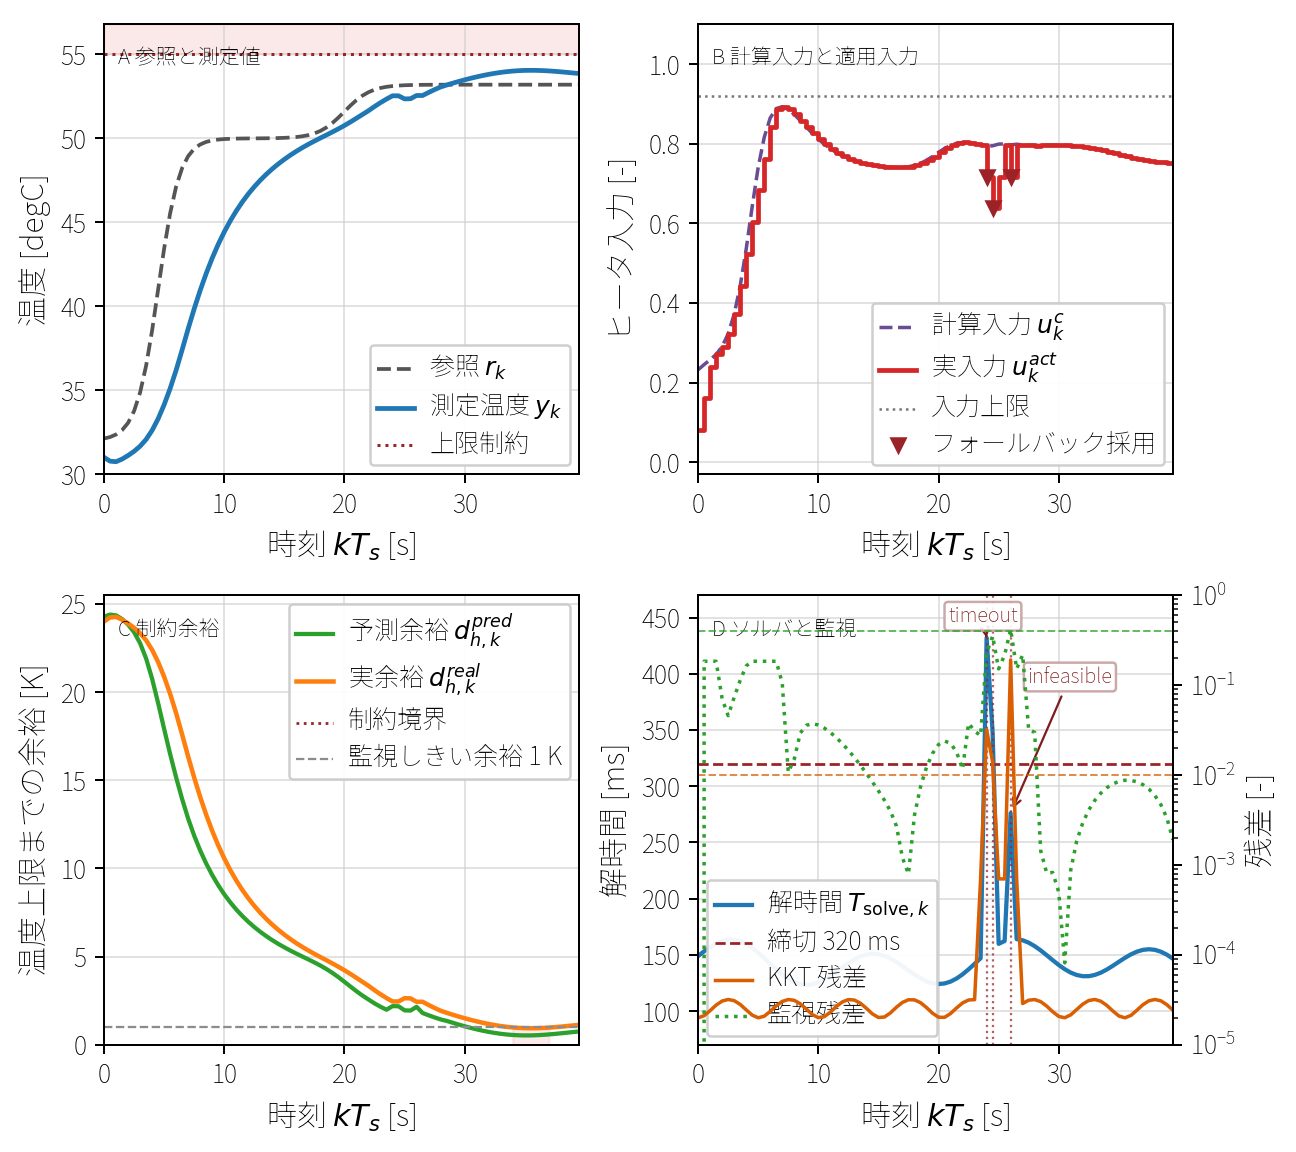
\includegraphics[width=0.96\linewidth,bb=0 0 1296 1152]{figures/validation_log_trace_examples.png}
  \caption[閉ループ実装検証ログの例]{制約付き温度制御を用いた閉ループ実装検証ログの例。参照と測定温度、計算入力と実入力、予測余裕と実余裕、解時間、KKT 残差、監視残差を同じ時刻列で比較している。}
  \label{fig:validation-log-trace-examples}
\end{figure}

\wfig{validation-log-trace-examples} では、$T_s=0.5\,\mathrm{s}$ の温度制御ログを 40 秒間だけ取り出している。上段左では、参照 $r_k$ が約 $53\,^\circ\mathrm{C}$ へ上がっても測定値 $y_k$ は上限 $55.0\,^\circ\mathrm{C}$ を越えていない。したがって、波形だけを見ると低リスク実機へ進めたくなる。しかし、下段右の解時間を見ると、$t=24.0\,\mathrm{s}$ で $T_{\mathrm{solve},k}=432\,\mathrm{ms}$、$t=24.5\,\mathrm{s}$ で $348\,\mathrm{ms}$ となり、締切 $320\,\mathrm{ms}$ を越えている。さらに、$t=26.0\,\mathrm{s}$ では終了状態が \texttt{infeasible} で、KKT 残差は $1.9\times10^{-1}$ まで上がる。解時間だけでなく終了状態と残差も同時に見なければ、「温度は制約内にある」という事実を正常な MPC 動作と誤って解釈してしまう。

このログで安全側に働いたのは、失敗周期で前回の入力を無条件に保持しなかったことである。$t=24.0\,\mathrm{s}$ では MPC の計算入力が $u_k^c=0.794$ であったのに対し、フォールバックとレート制限を通った実入力は $u_k^{act}=0.717$ であった。次の $t=24.5\,\mathrm{s}$ では $u_k^{act}=0.637$ まで下がり、$t=26.0\,\mathrm{s}$ の \texttt{infeasible} 周期でも $u_k^{act}=0.717$ が選ばれている。その結果、実余裕 $d_{h,k}^{\mathrm{real}}$ は失敗周期で約 $2.4\,\mathrm{K}$ 残り、全ログ中の最小値も $0.94\,\mathrm{K}$ で負になっていない。一方、監視残差は $t=26.0\,\mathrm{s}$ で $0.416$ となり、しきい値 $0.40$ を越える。これは、温度制約にはまだ触れていないが、通常モードとしては受け入れず、劣化運転または停止側へ遷移させるべき周期であることを示す。

したがって、このログは段階的ゲートの判定を二つに分ける。MIL の観点では、フォールバック則を含めた閉ループが温度上限を破らず、制約余裕が負にならないことは確認できる。SIL の観点では、実装コードが \texttt{timeout} と \texttt{infeasible} を未初期化入力へつなげず、指定されたフォールバック入力を出したことは確認できる。しかし、名目 MPC としては $T_{\mathrm{solve},k}\le320\,\mathrm{ms}$ と KKT 残差の受入条件を満たしていないため、このシナリオをそのまま HIL の通常運転試験へ進めてはならない。HIL へ進めるなら、通常性能の合格ログとしてではなく、ソルバ遅延と実行不可能状態を注入したフォールバック試験として扱い、同じ $r_k,y_k,u_k^c,u_k^{act},d_{h,k}^{\mathrm{real}},T_{\mathrm{solve},k},r_{\mathrm{mon},k}$ の列で、実制御計算機のタイマ、入出力更新、停止入力まで確認する。

段階的試験では、次の段階へ進む条件を安全ゲートとして定義する。段階 $q$ の合格フラグを $G_q$ とし、要求集合 $\mathcal{R}_q$、シナリオ集合 $\mathcal{S}_q$、ハード制約集合 $\mathcal{H}_q$ に対して
\begin{equation}
  G_q=1
  \Longleftrightarrow
  \begin{cases}
    \text{すべての } R_j\in\mathcal{R}_q \text{ に対応する受入基準が合格},\\
    \max_{\sigma_i\in\mathcal{S}_q,\ h\in\mathcal{H}_q,\ k} h(x_k)\le0,\\
    \max_k T_{\mathrm{solve},k}\le T_s-T_{\mathrm{margin}},\\
    \text{異常時モードと停止入力が指定時間内に作動}
  \end{cases}
\end{equation}
と置く。$G_q=0$ なら、次段階で調整して様子を見るのではなく、失敗した要求、シナリオ、ログ、設計仮定へ戻る。安全ゲートは保守的でよい。MIL で安全余裕が不足している制御器を SIL や HIL へ進めても、実装上の不具合と制御設計の不具合が重なり、原因が分からなくなる。

実機試験への進み方も段階化する。最初は対象を動かさない入出力確認で、センサの符号、単位、ゼロ点、入力方向、飽和、非常停止を確認する。次に、低エネルギーまたは狭い運転範囲で開ループまたは既存の低ゲイン制御により、同定で得たモデルと実測応答の差を見る。その後、監視器とフェイルセーフ入力を有効にしたまま、参照振幅、速度、外乱、運転範囲を少しずつ広げる。各段階では、試験前に停止条件を決め、試験中に監視し、試験後にログで受入基準を計算する。実機で初めて確認する項目は、できるだけ一つに絞る。制御器、推定器、配分、通信、機械条件を同時に変えると、不合格時に原因を分離できない。

最終的に、実機試験の合格は「一度うまく動いた」ことではなく、定義されたシナリオ集合で、要求に対応した受入基準を満たし、ログから安全余裕と時間余裕が確認でき、異常時の入力選択が設計通りに働いたことを意味する。制御工学の実装では、性能、制約、安全、計算時間、記録、仕様への追跡が一体である。これらを分けて検証し、最後に閉ループとして結合して確認することで、理論式を実対象へ移すときの危険な飛躍を小さくできる。

\wfig{mpc-architecture} の閉ループと \wfig{implementation-effects-examples} の実装差を同じ記録様式で追うと、段階的検証ゲートは次のように具体化できる。ここでは「軌跡がそれらしく見える」ことは合格条件にしない。次段階へ進む根拠は、制約違反、計算時間、ソルバ終了状態、監視残差、実入力 $u_k^{act}$ が数値の受入範囲に入っているというログ上の証拠である。

\begin{table}[tb]
  \centering
  \caption[段階的検証ゲートの例]{MIL、SIL、HIL、低リスク実機試験における段階的検証ゲートの例。}
  \begingroup
  \setlength{\tabcolsep}{2pt}
  \footnotesize
  \begin{tabular}{@{}>{\raggedright\arraybackslash}p{0.12\linewidth}>{\raggedright\arraybackslash}p{0.22\linewidth}>{\raggedright\arraybackslash}p{0.32\linewidth}>{\raggedright\arraybackslash}p{0.25\linewidth}@{}}
    \hline
    段階 & 確認する要求 & 合否判定量 & 次段階へ進めない失敗例 \\
    \hline
    MIL &
    同定モデルとセンサ・外乱モデルを含む閉ループで、全シナリオの状態制約と入力制約が守られる。 &
    $\max_{\sigma_i,j,k} h_j(x_k)\le0$、かつ追従 RMS 誤差 $e_{\mathrm{rms}}\le0.03\,\mathrm{m}$。 &
    狭い通路シナリオで $\max h_j(x_k)=0.012>0$ となり、安全余裕が消える。 \\
    SIL &
    実装コードが制御周期内に有効な入力を返し、推定器は指令値ではなく実入力 $u_k^{act}$ で更新される。 &
    ソルバ終了状態が全周期で \texttt{solved} または指定フォールバック、かつ $T_s=10\,\mathrm{ms}$ に対して $\max_k T_{\mathrm{solve},k}\le7\,\mathrm{ms}$。 &
    丸め誤差で制約行列が不整合になり、ソルバ終了状態が \texttt{infeasible} のまま前回入力を無条件に保持する。 \\
    HIL &
    制御計算機、入出力回路、通信、監視タスクを含めても実時間性と異常検知が成立する。 &
    $\max_k T_{\mathrm{solve},k}\le8\,\mathrm{ms}$、入出力更新ジッタ $\le1\,\mathrm{ms}$、監視残差 $r_{\mathrm{mon}}$ が断線注入後 $30\,\mathrm{ms}$ 以内にしきい値を越える。 &
    通信欠落時に $r_{\mathrm{mon}}$ が上がらず、停止入力へ遷移しない周期が 4 回続く。 \\
    低リスク実機 &
    低速・小振幅の運転範囲で、実入力、制約余裕、停止条件がログから確認できる。 &
    $\max_k \abs{u_k^{act}}\le u_{\mathrm{safe}}$、$\max_{j,k}h_j(\hat{x}_{k|k})\le0$、停止操作から $100\,\mathrm{ms}$ 以内に入力が 0 へ落ちる。 &
    見た目の追従は良くても、$u_k^{act}$ が電流制限に張り付き、制約余裕 $d_{h,k}^{\mathrm{real}}$ が負になる。 \\
    \hline
  \end{tabular}
  \endgroup
\end{table}

この対応表の各行は、段階ごとに一つの代表要求だけを示している。実際の試験票では、同じ形式で要求を増やし、合格した段階のログ、受入基準、ソフトウェア版、モデル識別子を結び付ける。重要なのは、MIL で制御設計の安全余裕不足を見つけ、SIL で実装差とソルバ扱いを見つけ、HIL で時間と入出力の仮定違反を見つけ、低リスク実機で実対象固有の入力・残差・停止挙動を小さな範囲で確認してから運転範囲を広げる、という順序を崩さないことである。
